\section{Strumentazione}
La strumentazione usata è quella presenta sul banco di lavoro, più:
\begin{itemize}
		\item alcuni circuiti integrati:
			\begin{enumerate}
			\item 2 IC SN74LS74 (Quad NAND Gate);
			\item 1 IC SN74LS93 (4-bit binary counter);
			\item 2 IC SN74LS74 (Dual D-Latch);
			\item 1 IC SN74LS86 (Quad XOR Gate);
			\end{enumerate}
		\item 1 DIP Switch a 4 interruttori;
		\item 1 pulsante a doppio contatto;
		\item 4 diodi LED;
		\item il generatore di onde quadre basato su Arduino realizzato precedentemente.
	\end{itemize}
\section{Flip-Flop D-Latch}
	Per realizzare un Flip-Flop D-Latch disponendo solo di NAND, è stato montato il circuito in \figurename{ \ref{f:D-Latch2}}.
	
	\begin{figure}[H]
		\centering
		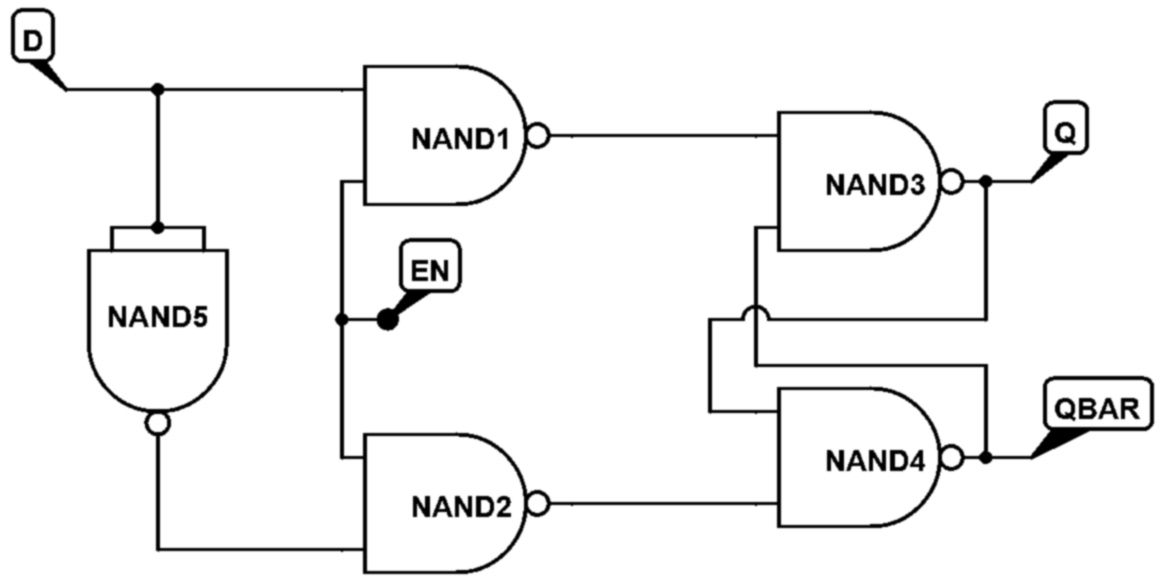
\includegraphics[scale=0.25]{ffdl.jpg}
		\caption{Schema del Flip-Flop D-Latch}
	\label{f:D-Latch2}
	\end{figure}
	L'ingresso D del circuito è stato collegato all'ingresso Y1 dell'impulsatore basato su arduino,
	mentre l'ingresso di ENABLE è stato collegato al dip switch in dotazione.
	Si è inoltre fornita una tensione di alimentazione continua $V_{cc}\sim\SI{5}{\volt}$.

	Per la verifica del funzionamento si è andati a verificare la tabella di verità riportata in \tablename{ \ref{t:D-Latch}} dove con il pedice 'prec' si intende che lo stato permanga nello stato precedente.
	\begin{table}[H]
		\centering
		\begin{tabular}{ssss}
			\toprule
			\text{$D$} & \text{$En$ }&\text{$Q$ }&\text{$\overline{Q}$}\\
			\midrule
			0 & 0 & Q_{prec} & {\overline{Q}}_{prec}\\
			1 & 0 & Q_{prec} & {\overline{Q}}_{prec}\\
			0 & 1 & 0 & 1\\
			1 & 1 & 1 & 0\\
			\bottomrule
		\end{tabular}
	\caption{Tabella di verità di un Flip-Flop D-Latch}
	\label{t:D-Latch}
	\end{table}
Per procedere alla verifica del funzionamento possiamo osservare gli output per mezzo di LED posti sulle uscite $Q$ e $\overline{Q}$ (con resistenze da $\sim \SI{330}{\ohm}$, per limitare la richiesta di corrente) o osservandoli direttamente all'oscilloscopio.

Si è collegato l' ingresso $En$ all'ingresso $Y2$ del generatore di onde quadre basato su Arduino. Essendo 	$Y1$ e 	$Y2$ sfasati di circa \ang{90}, in un periodo tali ingressi assumono tutte le possibili permutazioni di un ingresso a 2 bit.
Si riportano le acquisizioni ottenute in \fig{stocazzo} (si sono sovrapposte le letture per comodità di lettura, l'allineamento delle tracce è assicurato dall'uso del trigger sempre sullo stesso input).

	\begin{figure}[htb]
		\centering
		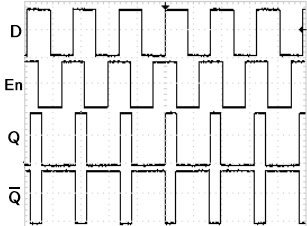
\includegraphics[scale=0.9]{ffdl_osc.jpg}
		\caption{Tabella di verità del Flip-Flop D-Lath vista all'oscilloscopio}
		\label{fig:stocazzo}
	\end{figure}
	
\paragraph{Misura dei tempi di ritardo}
	Essendo il circuito logico montato un sistema a più livelli
	si suppone che i tempi di ritardo tra il segnale in ingresso e quello in uscita non siano trascurabili, si è pertanto proceduto ad una misura dei tempi di propagazione per il fronte di salita e discesa del segnale.

	Si è usata un'onda quadra di frequenza $f=\SI{250.12\pm 0.01}{\hertz}$\footnote{Questa e tutte le seguenti misure di frequenza sono state eseguite con il frequenzimetro dell'oscilloscopio per via della sua grande precisione; si è preso fino all'ultima cifra stabile con il corrispondente errore.} all'ingresso $D$, mentre per la porta $En$ si è impiegato l'interruttore  posto normalmente sull'$1$ logico.

	Visualizzando l'andamento del segnale in $D$ e nelle uscite $Q$ e $\overline{Q}$
	sono stati misurati i seguenti ritardi:\\
	\begin{center}
		$\Delta t_{Q,salita}=\SI{16.4 \pm 0.1}{\ns} \qquad  \Delta t_{Q,discesa}=\SI{29.2 \pm 0.2}{\ns} $\\
		$\Delta t_{\overline{Q},salita}=\SI{29.2 \pm 0.2}{\ns} \qquad  \Delta t_{\overline{Q},discesa}=\SI{16.4 \pm 0.1}{\ns}$\\
	\end{center}

	Come è possibile osservare da i valori ottenuti $\Delta t_{\overline{Q},salita} = \Delta t_{{Q},discesa}$ e $\Delta t_{\overline{Q},discesa} = \Delta t_{{Q},salita}$; ciò risulta compatibile con le attese, essendo entrambe le uscite poste sul solito livello ed una l'inverso dell'altro.
	\paragraph{Note}
	Come riportato in \figurename{ \ref{f:D-Latch2}} per la realizzazione del Flip-Flop D-Latch in esame si è impiegato una porta NOT (ottenuto con la porta NAND5);
	tale porta svolge la funzione di inviare agli ingressi del Flip-Flop D-Latch valori opposti, permettendo di utilizzare quello che sarebbe altrimenti un gated SR-Latch come un level-triggered D-Latch.

	L'ingresso $En$ risulta essere attivo, e quindi abilita il circuito, per
	segnali in ingresso, in $En$, corrispondenti allo stato HIGH.

